%!TeX program = xelatex
\documentclass[12pt, oneside]{article}
\usepackage{amssymb,amsmath}
\usepackage[margin=1in]{geometry}
\usepackage{textpos}
\usepackage{float}
\usepackage{booktabs}
\usepackage{graphicx}
\usepackage[inter-unit-product =\cdot]{siunitx}
\let\DeclareUSUnit\DeclareSIUnit
\let\US\SI
\DeclareUSUnit\inch{in}
\DeclareUSUnit\foot{ft}
\DeclareUSUnit\mile{mi}
\DeclareUSUnit\foot{ft}
\DeclareUSUnit\slug{slug}
\DeclareUSUnit\pound{lb}
\DeclareUSUnit\psi{psi}
\DeclareUSUnit\Msi{Msi}
\DeclareUSUnit\ksi{ksi}

\begin{document}

\begin{textblock*}{4cm}(-1.7cm,-2.3cm)
\noindent {\scriptsize AE333 Fall 2021}
\end{textblock*}

\begin{textblock*}{8cm}(12.5cm,-1cm)
\noindent {Name: }
\end{textblock*}
\begin{textblock*}{13.5cm}(-1.7cm,-1.8cm)
\end{textblock*}

\vspace{1cm}

\begin{center}
\textbf{\Large Homework 8 Solutions}

\textbf{Due 19 November 2021}
\end{center}

\begin{enumerate}
	\item %9-17
		Find the stress state on an axis rotated $30^\circ$ counter-clockwise from the $x$ and $y$ axis.
		\begin{figure}[H]
			\centering
			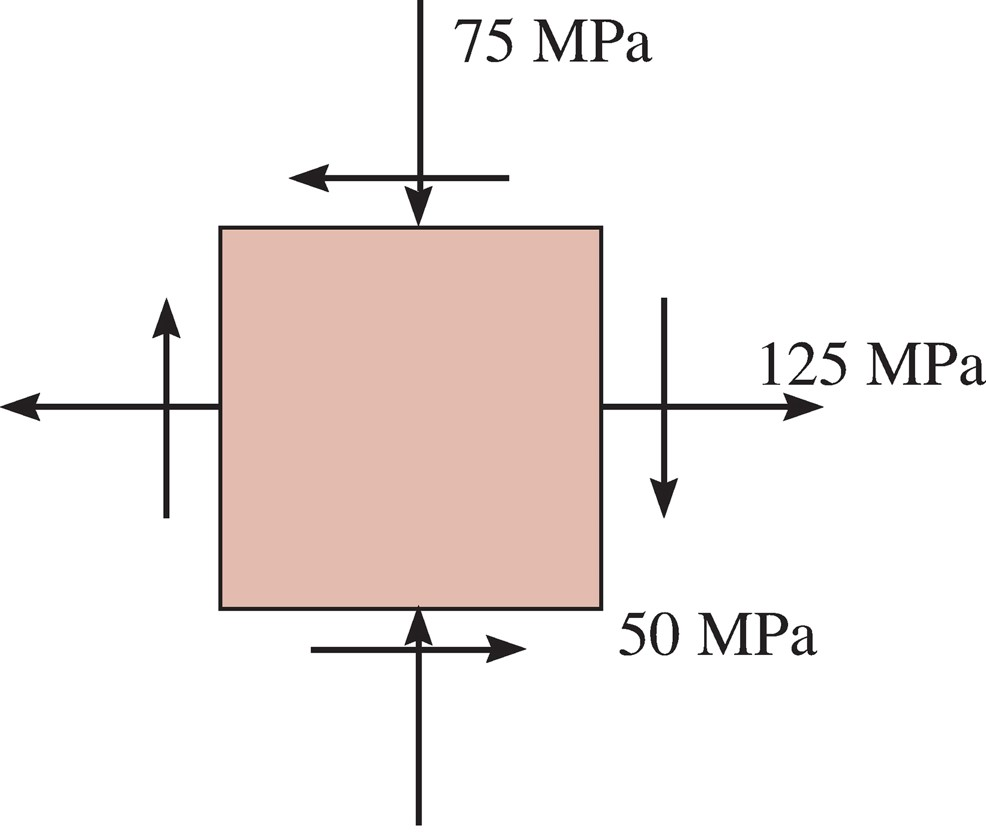
\includegraphics[width=0.6\linewidth]{9-17}
		\end{figure}
			\textbf{Solution:}
			\begin{itemize}
				\item There are three approaches that could be used to solve this problem, the first we discussed would be to section it and set up triangles, the second would be to use the general formulas and the third would be to use Mohr's circle.
					The most straight-forward to show in this solution is the formula, but you are free to use any method.
				\item 
$$\begin{aligned}
  \sigma_{x^\prime} &= \frac{\sigma_x+\sigma_y}{2} + \frac{\sigma_x-\sigma_y}{2} \cos 2\theta + \tau_{xy} \sin 2\theta \\
  \tau_{x^\prime y^\prime} &= - \frac{\sigma_x-\sigma_y}{2}\sin 2\theta + \tau_{xy} \cos 2\theta
\end{aligned}$$
				\item This gives $\sigma_{x^\prime} = 	\SI{31.7 }{MPa} $, $\sigma_{y^\prime} = 	\SI{18.3 }{MPa} $ and $\tau_{x^\prime y^\prime} = 	\SI{-111.6}{MPa} $
			\end{itemize}

	\item For the stress state in Problem 1, find the principal stresses and maximum (in-plane) shear stress
			\textbf{Solution:}
			\begin{itemize}
				\item Once again, we have a few different solutions, but we will continue using the formula
				\item 
$$\sigma_{1,2} = \frac{\sigma_x+\sigma_y}{2} \pm \sqrt {\left( \frac{\sigma_x-\sigma_y}{2}\right)^2 + \tau_{xy}^2}$$
				\item This gives $\sigma_1 = 	\SI{136.8}{MPa} $ and $\sigma_2 = 	\SI{-86.8}{MPa} $
				\item The maximum in plane shear stress is given by 
$$\tau_{max} = \sqrt{\left( \frac{\sigma_x-\sigma_y}{2} \right)^2 + \tau_{xy}^2}$$
				\item Which gives $\tau_{max} = 	\SI{111.8 }{MPa} $
			\end{itemize}

	\item %9-20
		The stress state along two planes is known as shown.
		Find the normal stresses on plane $b-b$ and the principal stresses.
		\begin{figure}[H]
			\centering
			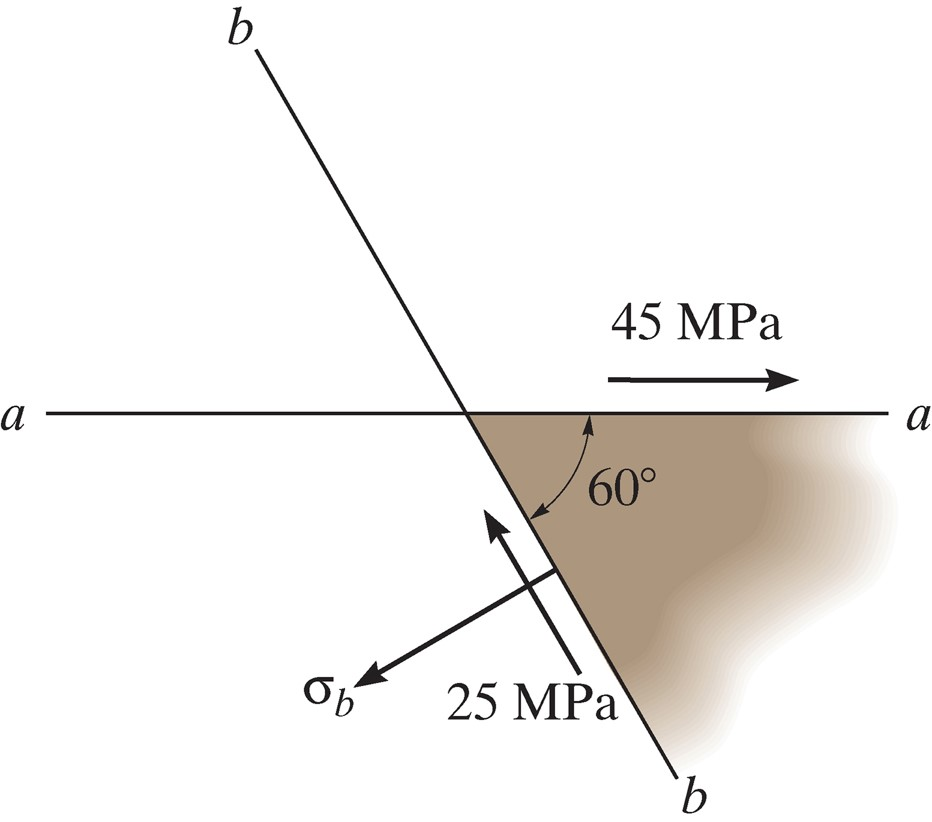
\includegraphics[width=0.6\linewidth]{9-20}
		\end{figure}
			\textbf{Solution:}
			\begin{itemize}
				\item We start by interpreting the problem a little bit, although they are not perpendicular, we can notice that the shear stresses shown for the $\tau_{xy}$ and $\tau_{ab}$ are acting in different directions, so whatever our convention, one of them should be negative while the other is positive.
        \item Next we use the formula for $\tau_{x^\prime y^\prime}$ with $x^\prime$ pointing in the same direction as $\sigma_b (\theta = 210^\circ)$
          \begin{equation} 
            -25 = -\left( \frac{\sigma_x - \sigma_y}{2} \right)\sin(420) + 45 \cos(420) 
          \end{equation}
				\item From the drawing we see that $\sigma_y = 0$, therefore we know $\sigma_x = \SI{109.7}{MPa} $, which we can now use to find $\sigma_b = \SI{121 }{MPa} $ 
				\item We can also find the principal stresses as $\sigma_1 = 	\SI{126 }{MPa} $ and $\sigma_2 = 	\SI{-16.1 }{MPa} $
			\end{itemize}

	\item %9-24
		The wood beam is subjected to a load of $ 	\SI{12 }{kN}  $.
		If grains of wood in the beam at point $A$ make an angle of $25^\circ$ with the horizontal as shown find the normal and shear stress that act perpendicular to the grains.
		\begin{figure}[H]
			\centering
			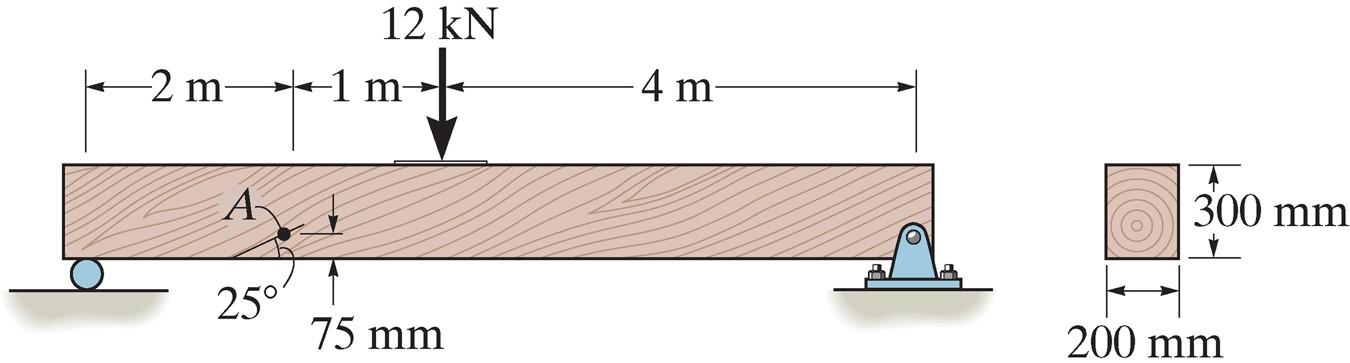
\includegraphics[width=0.8\linewidth]{9-24}
		\end{figure}
			\textbf{Solution:}
			\begin{itemize}
				\item We first need to use the flexure and transverse shear formulas to find the stress state at point $A$
				\item Starting with statics, we find the left reaction force to be $F_1 = 	\SI{6.86}{kN} $ and the right reaction force $F_2 = 	\SI{5.14}{kN} $
				\item This gives $V = 	\SI{6.86}{kN} $ and $M = 	\SI{13.71}{kN.m} $ at $A$
				\item For the cross section we find $I = 	\SI{450e6}{mm^4} $
				\item At $A$ we have $y = 	\SI{75}{mm} $
				\item To calculate $Q$ we find $\bar{A} = 	\SI{15e3}{mm^2} $ and $\bar{y} = 	\SI{112.5 }{mm} $ which gives $Q = 	\SI{1.688}{mm^3} $
				\item This gives a stress state of $\sigma_x = 	\SI{2.286}{MPa} $ and $\tau_{xy} = 	\SI{128.6 }{Pa} $
				\item To find the normal and shear stresses in the direction of the wood fibers, we use the stress transformation equations with $\theta = 25^\circ$
				\item We find $\sigma_{x^\prime} = 	\SI{1.98}{MPa} $ (in the fiber direction) and $\sigma_{y^\prime} = 	\SI{0.31}{MPa} $ (perpendicular to the fiber direction) and $\tau_{x^\prime y^\prime} = 	\SI{-0.79}{MPa} $
			\end{itemize}

	\item Draw Mohr's circle for the stress state in problem 4 and use it to estimate the principal stresses.
			\textbf{Solution:}
			\begin{itemize}
				\item Here we will ignore the work done previously and draw mohr's circle directly for the initial stress state, $\sigma_x = 	\SI{2.286 }{MPa} $, $\sigma_y = 	\SI{0}{MPa} $ and $\tau_{xy} = 	\SI{0.129}{MPa} $
					\begin{figure}[H]
						\centering
						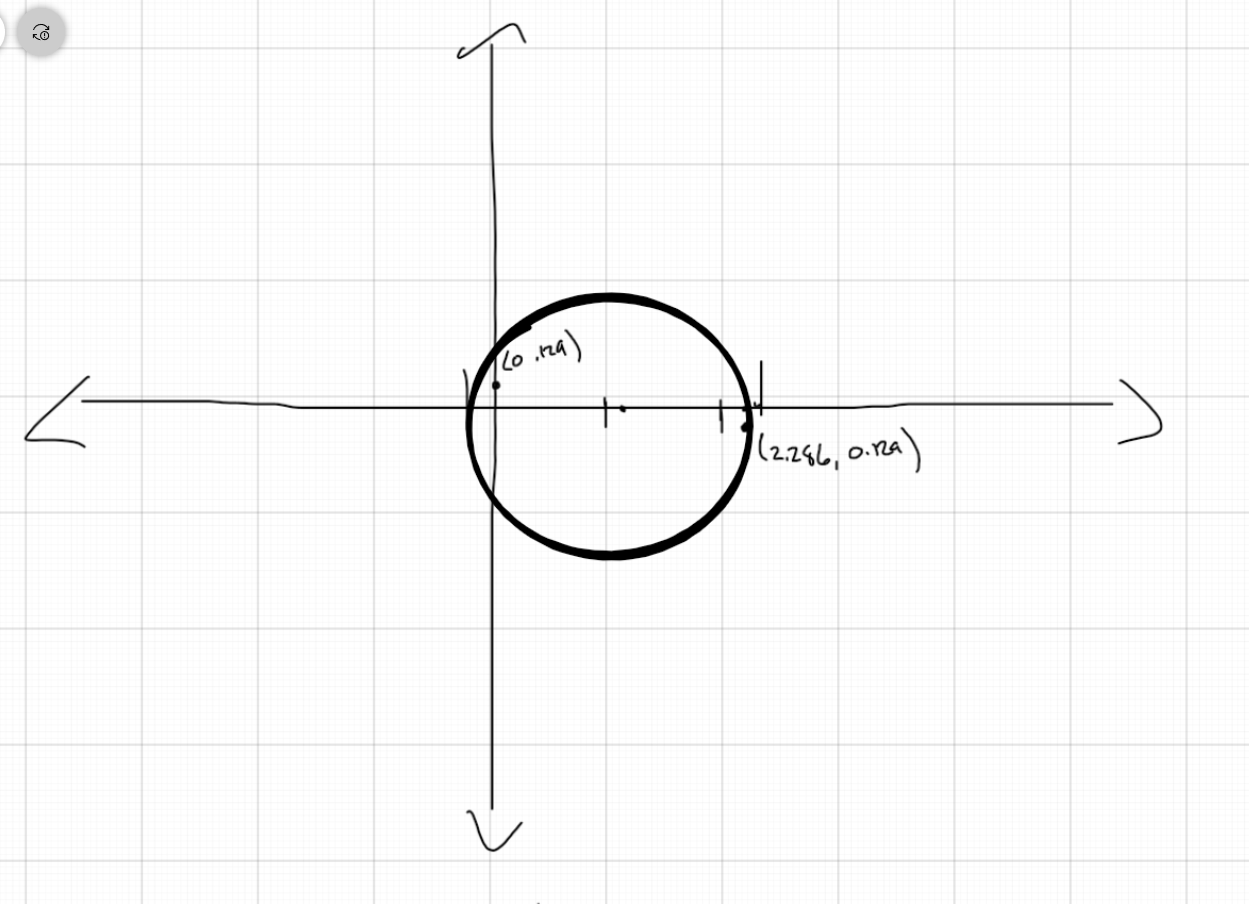
\includegraphics[width=0.6\linewidth]{mohr}
					\end{figure}
				\item Although my digital drawing is not ideal, it is clear to see that the principal stresses will be fairly close to the current stress state, with perhaps $\sigma_1 = 	\SI{2.4 }{MPa} $ and $\sigma_2 = 	\SI{-0.1}{MPa} $
			\end{itemize}

	\item %10-25
		The $45^\circ$ strain rosette is mounted on the surface of a shell with the following readings: $\epsilon_a = -200 \mu \epsilon$, $\epsilon_b = 300 \mu \epsilon$ and $\epsilon_c = 250 \mu \epsilon$.
		Find the in-plane principal strains.
		\begin{figure}[H]
			\centering
			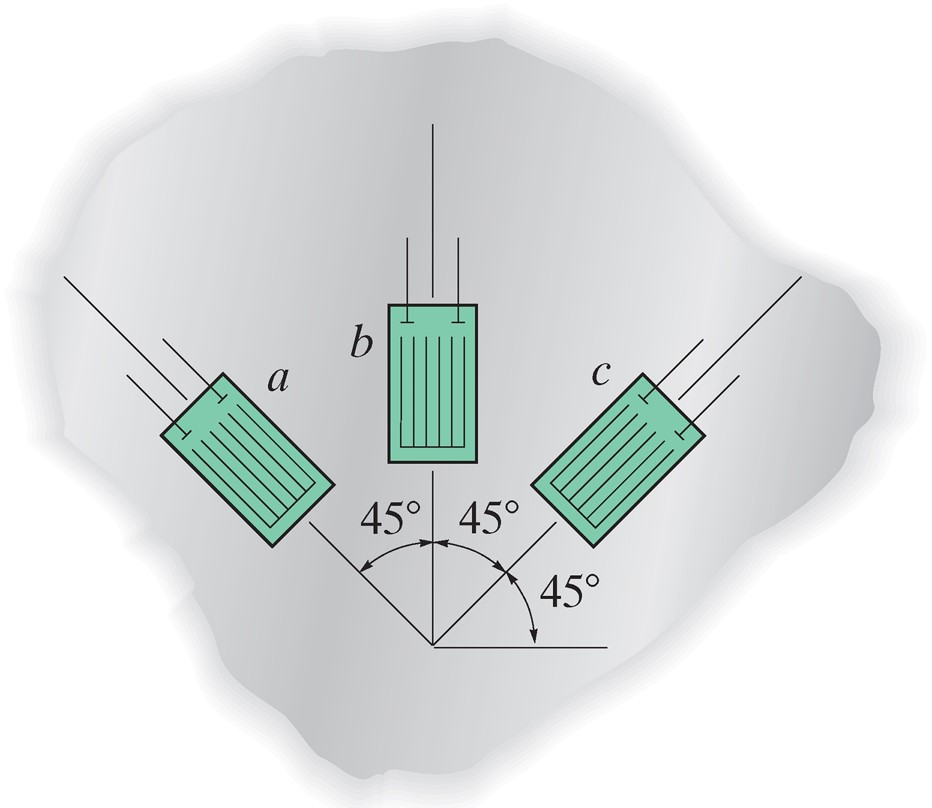
\includegraphics[width=0.6\linewidth]{10-25}
		\end{figure}
			\textbf{Solution:}
			\begin{itemize}
				\item From the figure, we can see that $\epsilon_b = \epsilon_y$, the other strain measurements we will need to find using the strain transformation equations.
					\[\epsilon_{x^\prime} = \frac{\epsilon_x+\epsilon_y}{2} + \frac{\epsilon_x-\epsilon_y}{2} \cos 2\theta + \frac{\gamma_{xy}}{2} \sin 2\theta \]
				\item If we set up the equations for the two angles we have left, $\theta_a = 45^\circ$ and $\theta_c = 135^\circ$
					\[ \begin{aligned}
						\epsilon_{a} &= \frac{\epsilon_x+\epsilon_y}{2} + \frac{\epsilon_x-\epsilon_y}{2} \cos 2\theta_a + \frac{\gamma_{xy}}{2} \sin 2\theta_a \\
					\epsilon_{c} = \frac{\epsilon_x+\epsilon_y}{2} + \frac{\epsilon_x-\epsilon_y}{2} \cos 2\theta_c + \frac{\gamma_{xy}}{2} \sin 2\theta_c 
					\end{aligned}\]
				\item Note that $\sin(2\theta_a)=1$, $\sin(2\theta_c)=-1$, $\cos(2\theta_a)=0$, and $\cos(2\theta_c)=0$
					\[ \begin{aligned}
						-200 \mu \epsilon &= \frac{\epsilon_x+300 \mu \epsilon}{2} + \frac{\gamma_{xy}}{2} \\
						250 \mu \epsilon &= \frac{\epsilon_x+300 \mu \epsilon}{2} - \frac{\gamma_{xy}}{2} 
					\end{aligned}\]
				\item From which we find that $\epsilon_x = -250 \mu \epsilon$ and $\gamma_{xy} = -225 \mu \epsilon$
			\end{itemize}

	\item %10-45
		A material is subjected to principal stresses $\sigma_x$ and $\sigma_y$.
		Find the orientation, $\theta$, of the strain gage so that its reading of normal strain corresponds only to $\sigma_y$, not $\sigma_x$.
		The relevant material constants for this problem are $E$ and $\nu$ (express answer in terms of these)
		\begin{figure}[H]
			\centering
			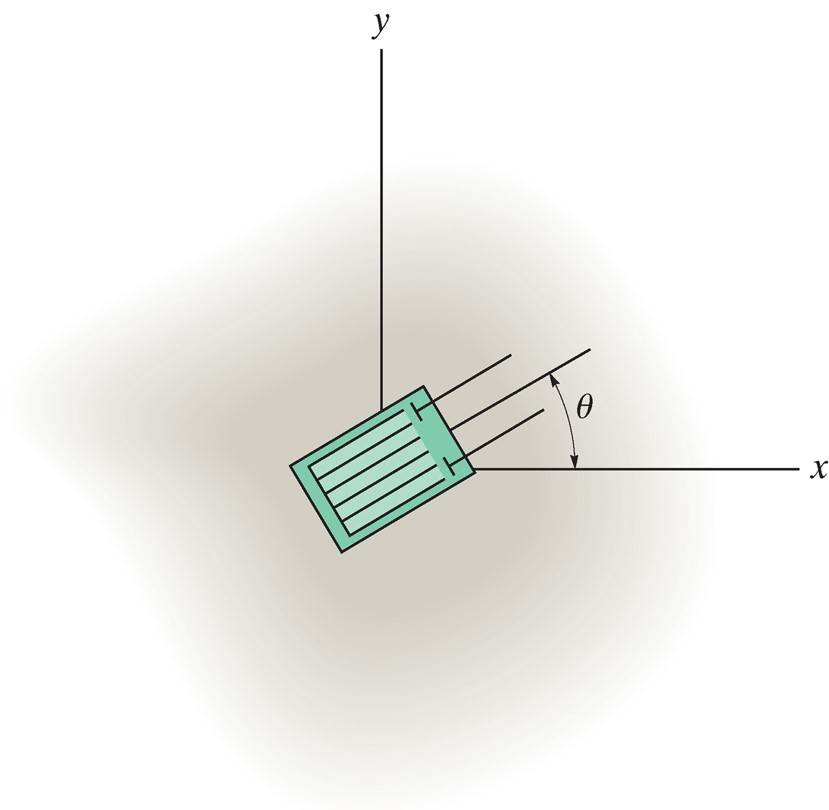
\includegraphics[width=0.6\linewidth]{10-45}
		\end{figure}
			\textbf{Solution:}
			\begin{itemize}
				\item Notice that the problem states we have applied principal stresses, this means that in this plane there are no shear stresses applied
				\item The reason we cannot simply align the strain gage in the $y$-direction is that this would include some Poisson's contraction from stress in the $x$-direction.
				\item We start by writing the equation for $\sigma_{x^\prime}$ and $\sigma_{y^\prime}$ in the direction of our strain gage.
					For no shear stress it is more convenient to substitute $\cos 2\theta = 2\cos^2 \theta -1$ which gives
					\[ \begin{aligned}
						\sigma_{x^\prime} &= \sigma_x \cos^2\theta + \sigma_y \sin^2 \theta\\
						\sigma_{y^\prime} &= \sigma_x \sin^2\theta + \sigma_y \cos^2 \theta
					\end{aligned}\]
				\item We can now write an expression for $\epsilon_{x^\prime}$ using Hooke's Law (and neglecting out-of-plane terms)
					\[ \epsilon_{x^\prime} = \frac{1}{E}( \sigma_{x^\prime} - \nu \sigma_{y^\prime} )\]
				\item Substituting the previous equations for $\sigma_{x^\prime}$ and $\sigma_{y^\prime}$ gives
					\[ \epsilon_{x^\prime} = \frac{1}{E}( \sigma_x \cos^2\theta + \sigma_y \sin^2 \theta - \nu [\sigma_x \sin^2\theta + \sigma_y \cos^2 \theta)]\]
				\item To eliminate $\sigma_x$ from this equation we need $\sigma_x \cos^2\theta - \nu \sigma_x \sin^2 \theta = 0$
				\item Factoring $\sigma_x$ we have 
					\[ \sigma_x ( \cos^2\theta - \nu \sin^2\theta = 0 )\]
				\item To solve for any $\sigma_x$ we set the portion in parentheses equal to 0 and solve for $\theta$, which gives $\theta = \tan^{-1}\left( \frac{1}{\sqrt{\nu}} \right)$
			\end{itemize}

\end{enumerate}
\end{document}
